\section{Feldman-Cousins comparison with p-theta}
\label{app:fc_compare}

This section presents comparisons of VALOR and p-theta Feldman-Cousins critical values obtained by each group. The agreement between the two groups is generally good for both mass orderings.

\begin{figure*}[htb]
	\center
	\begin{subfigure}[b]{\textwidth}
		\center
		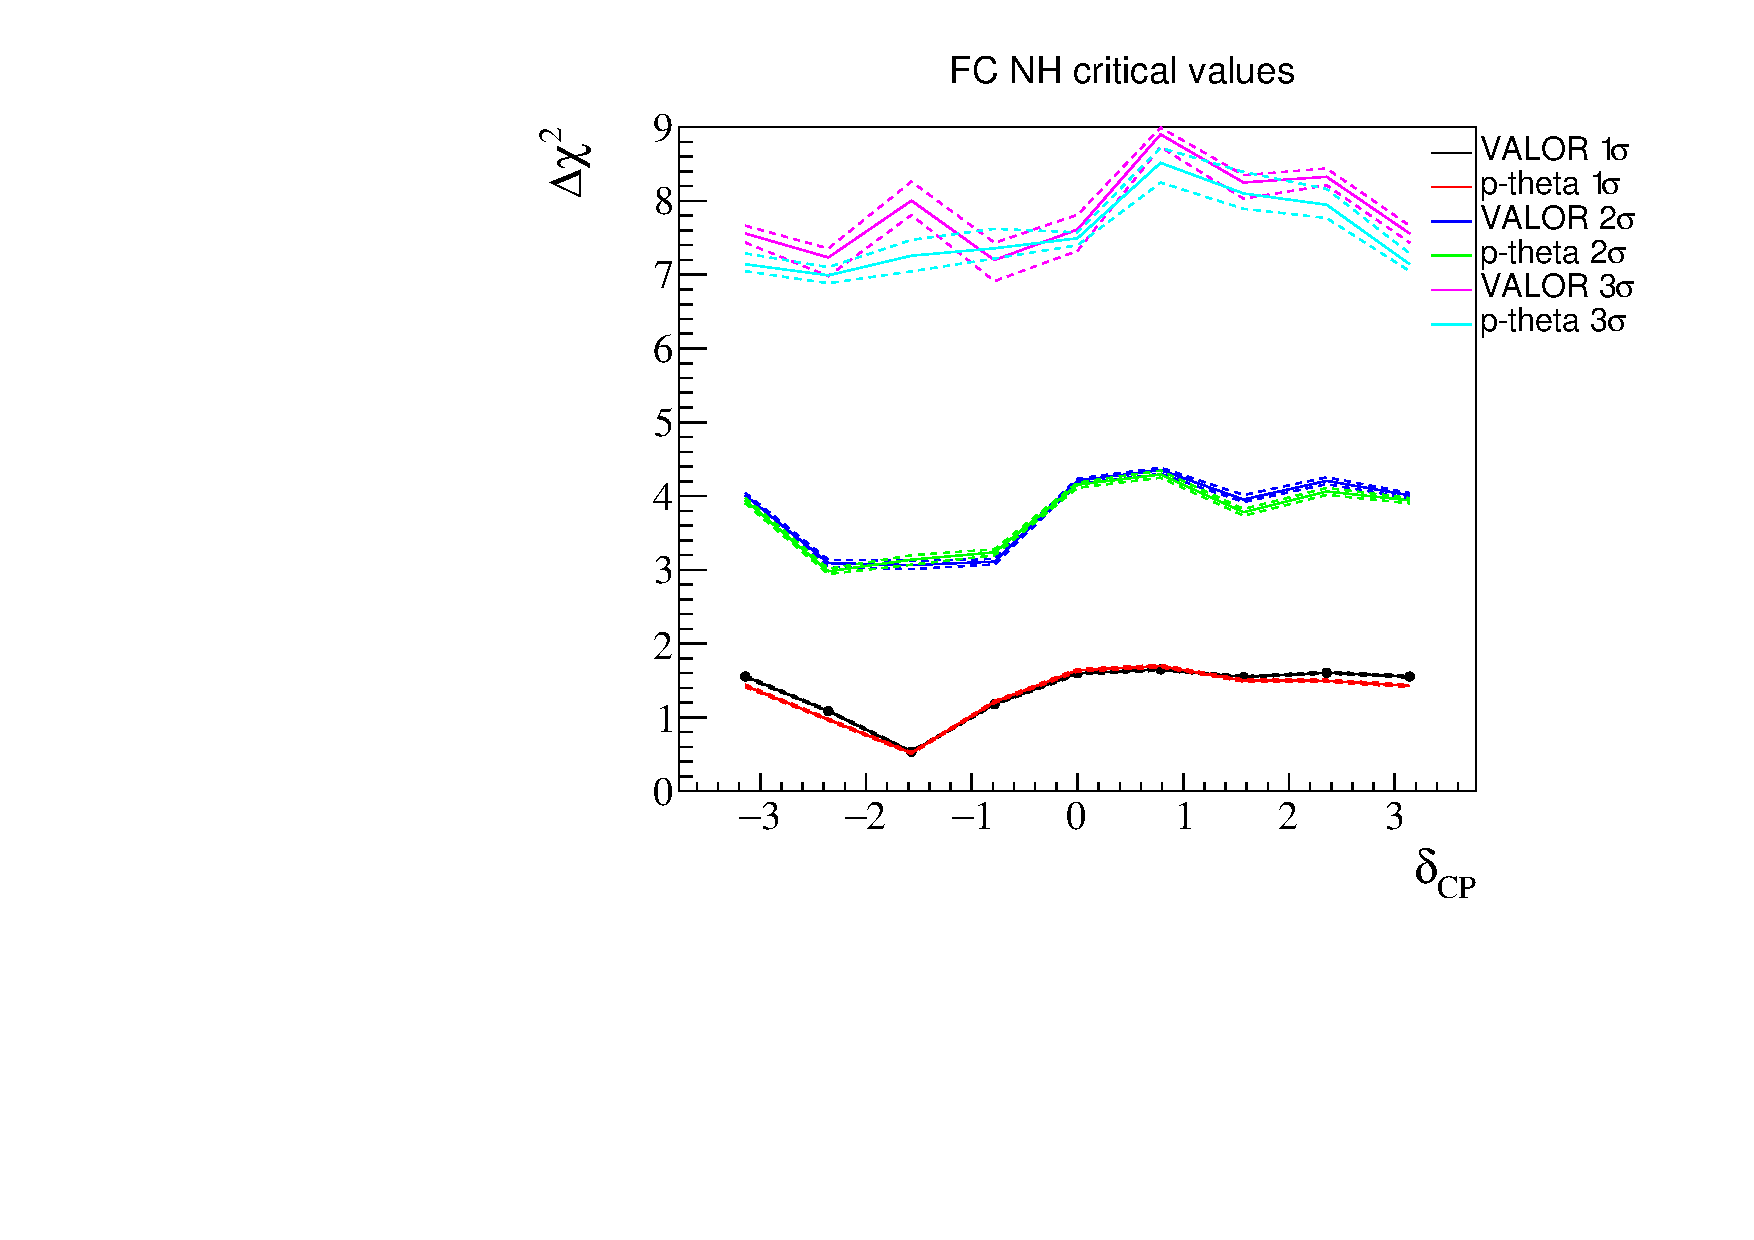
\includegraphics[width=0.68\textwidth, page=1]{images/fc/fc_compare}
		\caption{Normal ordering}
	\end{subfigure}
	\begin{subfigure}[b]{\textwidth}
		\center
		\includegraphics[width=0.68\textwidth, page=2]{images/fc/fc_compare}
		\caption{Inverted ordering}
	\end{subfigure}
	\caption {
		Feldman-Cousins critical values.
	}
	\label{fig:fc_cv_compare}
\end{figure*}

\clearpage